\documentclass[11pt]{article}
\usepackage[T1]{fontenc}
\usepackage[utf8]{inputenc}
\usepackage[margin=1in]{geometry}
\usepackage{amsmath,amssymb}
\usepackage{booktabs}
\usepackage{array}
\usepackage{tabularx}
\usepackage{graphicx}
\usepackage{float}
\usepackage{hyperref}
\usepackage[round,authoryear]{natbib}

% Generated by scripts/build_tex_values.py. Do not edit by hand.
\newcommand{\AnalysisDigest}{7970e74de0a5868bc3d608fb07daf2fcec333bc019b095530e42371730ee9a4a}
\newcommand{\SourceDigest}{6a5275a85358c7e2e42fc16db1fdd746f7ba8e4d249e8e91b4fa26b18f530b55}
\newcommand{\DesignTasks}{30}
\newcommand{\DesignCandidates}{3}
\newcommand{\GeneratorModel}{llama3.2:3b}
\newcommand{\SelectorModel}{qwen2.5:7b}
\newcommand{\SampleSeed}{20261023}
\newcommand{\BootstrapDraws}{20000}
\newcommand{\BootstrapSeed}{20261027}
\newcommand{\OrderContractDiffer}{26}
\newcommand{\OriginalHardOrderMismatchTasks}{23}
\newcommand{\HardRepairPickChangedTasks}{11}
\newcommand{\DuplicateAnswerTasks}{5}
\newcommand{\ScoreAContentChanged}{7}
\newcommand{\ScoreBContentChanged}{5}
\newcommand{\OrderNoScoreContentChanged}{14}
\newcommand{\OrderScoreContentChanged}{14}
\newcommand{\OrderNoScoreSameContentSlot}{1}
\newcommand{\OrderScoreSameContentSlot}{0}
\newcommand{\ScoreASameContentSlot}{0}
\newcommand{\ScoreBSameContentSlot}{0}
\newcommand{\ScoreAChoiceChanged}{7}
\newcommand{\ScoreAChoicePairs}{30}
\newcommand{\ScoreAChoiceRate}{23.3\%}
\newcommand{\ScoreAChoiceCI}{11.8\% to 40.9\%}
\newcommand{\ScoreAScoreDelta}{+0.0444}
\newcommand{\ScoreAScoreDeltaCI}{+0.0000 to +0.1222}
\newcommand{\ScoreAScorePairs}{30}
\newcommand{\ScoreAScoreIncreased}{2}
\newcommand{\ScoreAScoreUnchanged}{28}
\newcommand{\ScoreAScoreDecreased}{0}
\newcommand{\ScoreBChoiceChanged}{5}
\newcommand{\ScoreBChoicePairs}{30}
\newcommand{\ScoreBChoiceRate}{16.7\%}
\newcommand{\ScoreBChoiceCI}{7.3\% to 33.6\%}
\newcommand{\ScoreBScoreDelta}{+0.0667}
\newcommand{\ScoreBScoreDeltaCI}{+0.0000 to +0.1667}
\newcommand{\ScoreBScorePairs}{30}
\newcommand{\ScoreBScoreIncreased}{2}
\newcommand{\ScoreBScoreUnchanged}{28}
\newcommand{\ScoreBScoreDecreased}{0}
\newcommand{\OrderNoScoreChoiceChanged}{15}
\newcommand{\OrderNoScoreChoicePairs}{30}
\newcommand{\OrderNoScoreChoiceRate}{50.0\%}
\newcommand{\OrderNoScoreChoiceCI}{33.2\% to 66.8\%}
\newcommand{\OrderNoScoreScoreDelta}{-0.0222}
\newcommand{\OrderNoScoreScoreDeltaCI}{-0.1000 to +0.0333}
\newcommand{\OrderNoScoreScorePairs}{30}
\newcommand{\OrderNoScoreScoreIncreased}{1}
\newcommand{\OrderNoScoreScoreUnchanged}{28}
\newcommand{\OrderNoScoreScoreDecreased}{1}
\newcommand{\OrderScoreChoiceChanged}{14}
\newcommand{\OrderScoreChoicePairs}{30}
\newcommand{\OrderScoreChoiceRate}{46.7\%}
\newcommand{\OrderScoreChoiceCI}{30.2\% to 63.9\%}
\newcommand{\OrderScoreScoreDelta}{+0.0000}
\newcommand{\OrderScoreScoreDeltaCI}{+0.0000 to +0.0000}
\newcommand{\OrderScoreScorePairs}{30}
\newcommand{\OrderScoreScoreIncreased}{0}
\newcommand{\OrderScoreScoreUnchanged}{30}
\newcommand{\OrderScoreScoreDecreased}{0}
\newcommand{\ExposedTop}{60}
\newcommand{\ExposedSlots}{60}
\newcommand{\ExposedInvalidSlots}{0}
\newcommand{\ExposedNontiedTop}{12}
\newcommand{\ExposedNontiedSlots}{12}
\newcommand{\AllTiedInstrumentTasks}{24}
\newcommand{\VariedInstrumentTasks}{6}
\newcommand{\OrderAAllTiedTasks}{24}
\newcommand{\OrderAAllTiedChoiceChanged}{5}
\newcommand{\OrderAAllTiedChoiceRate}{20.8\%}
\newcommand{\OrderAAllTiedScoreDelta}{+0.0000}
\newcommand{\OrderAVariedTasks}{6}
\newcommand{\OrderAVariedChoiceChanged}{2}
\newcommand{\OrderAVariedChoiceRate}{33.3\%}
\newcommand{\OrderAVariedScoreDelta}{+0.2222}
\newcommand{\OrderBAllTiedTasks}{24}
\newcommand{\OrderBAllTiedChoiceChanged}{3}
\newcommand{\OrderBAllTiedChoiceRate}{12.5\%}
\newcommand{\OrderBAllTiedScoreDelta}{+0.0000}
\newcommand{\OrderBVariedTasks}{6}
\newcommand{\OrderBVariedChoiceChanged}{2}
\newcommand{\OrderBVariedChoiceRate}{33.3\%}
\newcommand{\OrderBVariedScoreDelta}{+0.3333}

\graphicspath{{figures/}}
\hypersetup{hidelinks}

\title{Auditing Score Exposure and Presentation Order\\
in LLM Harness Selection: A Matched 30-Task Case Study}
\author{Zewen Liu\\Independent Researcher}
\date{}

\begin{document}
\raggedbottom
\emergencystretch=2em
\maketitle

\begin{abstract}
Harness evaluations often choose among candidate outputs and then report a score for the chosen
candidate. The interface used to make that choice is part of the measurement: a selector may see the
grader's score, one of several presentation orders, or both. We conducted a within-task
\(2\times2\) audit on a frozen local benchmark, with three fixed candidate answers per task and four
selection arms that crossed two orders with hidden or visible rubric scores. The audit used
\DesignTasks{} tasks, a \GeneratorModel{} candidate generator, and a \SelectorModel{} selector.

Exposing scores while holding order A fixed changed the selected candidate on
\ScoreAChoiceChanged/\ScoreAChoicePairs{} tasks (\ScoreAChoiceRate; Wilson 95\% CI
\ScoreAChoiceCI). The corresponding result under order B was
\ScoreBChoiceChanged/\ScoreBChoicePairs{} (\ScoreBChoiceRate; CI \ScoreBChoiceCI). Changing order with
scores hidden changed the selected slot on \OrderNoScoreChoiceChanged/\OrderNoScoreChoicePairs{}
tasks (\OrderNoScoreChoiceRate; CI \OrderNoScoreChoiceCI); changing order with scores visible produced
\OrderScoreChoiceChanged/\OrderScoreChoicePairs{} (\OrderScoreChoiceRate; CI \OrderScoreChoiceCI).
Every changed score-exposure choice selected different answer text. Across the two order contrasts,
the counts of slot changes that selected byte-identical text were
\OrderNoScoreSameContentSlot{} with scores hidden and \OrderScoreSameContentSlot{} with scores visible.

The deterministic rubric most often could not distinguish the selected outputs: all three candidates
tied on \AllTiedInstrumentTasks/\DesignTasks{} tasks. Score exposure nevertheless changed the selected
slot on \OrderAAllTiedChoiceChanged/\OrderAAllTiedTasks{} all-tied tasks under order A and
\OrderBAllTiedChoiceChanged/\OrderBAllTiedTasks{} under order B (Table~\ref{tab:ties}). When scores
were visible, the selector chose a top-scored
candidate in \ExposedTop/\ExposedSlots{} arm-task slots. These results are a reproducible interface
audit, not evidence that the rubric measures answer quality or that the observed rates generalise to
other models and task populations.
\end{abstract}

\section{Introduction}

Evaluating an LLM agent harness usually involves more than running one fixed program. A pipeline may
generate several candidates, choose one, and score the choice. Selection bias when a selected
candidate is subsequently evaluated on the same evidence is a classical concern
\citep{cawley2010overfitting}, and adaptive reuse of evaluation data can break the nominal validity
of intervals and tests \citep{dwork2015holdout}. LLM evaluation adds another interface: the chooser
can be an LLM that is sensitive to the way candidates are presented.

Two manipulations are easy to overlook because both leave the candidate answers unchanged. First,
the selector can be shown the grader's score. If that score is also the reported outcome, the
selection and measurement stages are no longer independent. Second, candidate order can change.
Position effects in LLM judges are well documented \citep{shi2024judgingjudges}, so an uncontrolled
order difference can move choices even when no score is exposed.

We ask a narrow question. For a fixed candidate pool, how often does each manipulation change the
selected slot, the selected answer text, and the selected candidate's rubric score? We answer it with
one matched case study rather than a population estimate. The same three candidates enter a
\(2\times2\) design: order A or B, crossed with hidden or visible rubric scores. This lets us form two
score-exposure contrasts and two order contrasts without comparing the diagonal in which both
factors change.

The contribution is an auditable empirical record:
\begin{itemize}
\item the exact candidate pool is shared across all four arms;
\item presentation order is reconstructed from the frozen runner and checked against the analysis;
\item every one of the 90 raw answer files is hashed, and every stored rubric score is recomputed;
\item the paper reports slot changes, answer-content changes, and rubric-score changes separately;
\item the score-exposure and order contrasts are presented under both levels of the other factor.
\end{itemize}

We do not claim a new estimator or a universal harness bias. The useful evidence is that a fixed
candidate pool can produce materially different selections under two interface variations, while the
benchmark's deterministic rubric often registers no score difference at all.

\section{Related Work}

\paragraph{Selection and evaluation reuse.}
The winner's-curse problem in model selection arises when the noisy measurement used to choose a
candidate is also treated as an unbiased evaluation of that candidate
\citep{cawley2010overfitting}. Reusable-holdout methods address a related problem in adaptive data
analysis: repeated choices made using the same evidence can overfit that evidence
\citep{dwork2015holdout}. Our design separates the two visible input factors before selection, but it
does not provide the fresh-task holdout that would validate a deployment claim.

\paragraph{Presentation and preference leakage.}
Studies of LLM-as-a-judge systems identify position, verbosity, and self-enhancement effects
\citep{gu2025judgesurvey,shi2024judgingjudges}. Preference leakage further shows that the relation
between the generator and judge can affect judge outputs \citep{li2025preference}. Work on strict
estimator separation motivates care when the same information or model family participates in both
choosing and evaluating \citep{nahhas2026estimator}. Our score-visible arm is a direct, deliberately
visible interface leak rather than an inferred preference relation. The order contrast is included as
a separate manipulation.

\paragraph{Harness evaluation.}
Recent agent-evaluation work treats the surrounding harness as a hidden variable rather than a
constant. Harness search and recursive harness construction make the harness an object of
optimisation \citep{xu2026harness2}; other work argues that agent comparisons must disclose the
harness \citep{zhang2026disclose}, studies scaffold choice as part of the effective system
\citep{vats2026scaffold}, and examines how harness evolution should be evaluated
\citep{harness2026rethinking}. Our audit addresses a lower-level interface question within such an
evaluation: what happens when the same candidates are chosen under different score visibility and
order.

\paragraph{Estimands and construct validity.}
Evaluation results are difficult to interpret when the target quantity and the measurement
procedure are not separated \citep{binette2024estimands,freiesleben2025epistemology}. We therefore
report the estimator explicitly: the fraction of paired tasks on which the selected slot changes,
the fraction on which selected answer content changes, and the paired difference in the selected
candidate's rubric score. The rubric is an outcome measure, not an independent estimate of answer
quality.

\section{Audit Design}

\subsection{Frozen task and candidate pool}

We used the development subset of a local WSE-Bench manifest. The frozen run sampled
\DesignTasks{} tasks with seed \SampleSeed. For each task, the generator produced
\DesignCandidates{} candidate answers from preset harness variants and wrote them to persistent files.
The candidate generator was the local Ollama alias \texttt{\GeneratorModel}; the selector was the
local alias \texttt{\SelectorModel}. Candidate generation used a low fixed temperature, and selection
used deterministic decoding. The post-run installed model records are retained as artifacts; the
runner itself did not persist the response's model digest.

The same three raw answers enter every selection arm. Before analysis, we verified that all
\DesignTasks{} \(\times\) \DesignCandidates{} expected answer files existed. This prevents an arm from
silently sampling a fresh candidate after the intervention.

\subsection{The \texorpdfstring{\(2\times2\)}{2x2} selection interface}

Table~\ref{tab:design} shows the four arms. Order A and order B are deterministic, mode-specific
permutations of the candidate indices. They are stable across reruns but differ on
\OrderContractDiffer/\DesignTasks{} tasks. Only within-row and within-column pairs are used. The
diagonal that changes both order and score visibility is excluded.

A code audit found that the original runner seeded the visible-score order-B arm from the literal
mode name rather than from the score-hidden order-B arm. The two permutations differed on
\OriginalHardOrderMismatchTasks{} of \DesignTasks{} tasks. We therefore preserved the original run and
replayed only that arm with the frozen candidates, scores, selector settings, and intended order B.
The repair changed \HardRepairPickChangedTasks{} selected candidates; all manuscript outcomes use the
replayed record. The other three arms were reused byte-for-byte, and each replay response is stored
with its prompt and response hashes.

\begin{table}[H]
\centering
\small
\begin{tabular}{@{}lll@{}}
\toprule
 & \textbf{Scores hidden} & \textbf{Scores visible} \\
\midrule
\textbf{Order A} & \texttt{honest} & \texttt{hard\_a} \\
\textbf{Order B} & \texttt{honest\_shuffled} & \texttt{hard} \\
\bottomrule
\end{tabular}
\caption{The observed \(2\times2\) selection design. Score-exposure contrasts compare left and right;
order contrasts compare top and bottom. The one order pair is a control in this run, not a balanced
sample of all possible permutations.}
\label{tab:design}
\end{table}

\subsection{Outcomes}

For each paired contrast, we report:
\begin{enumerate}
\item whether the selected candidate index changed;
\item whether the selected raw answer's SHA-256 changed, which avoids treating duplicate text as a
content change;
\item the deterministic rubric score of the selected candidate before and after the manipulation.
\end{enumerate}

Choice-change proportions use a Wilson score interval. Mean selected-score differences use a
paired-task percentile bootstrap with \BootstrapDraws{} draws and seed \BootstrapSeed. These intervals
describe uncertainty over the frozen task sample; they do not turn the case study into a population
estimate. Candidate content was generated once per task and reused unchanged.

\subsection{Integrity checks}

The analysis and evidence are generated from the frozen runner output, not copied manually into the
paper. We independently recomputed all 90 rubric scores from the raw answers with the evaluator code
and obtained zero mismatches. The source JSON hash is:
\begin{flushleft}\ttfamily\small\SourceDigest\end{flushleft}
The deterministic analysis artifact hash is:
\begin{flushleft}\ttfamily\small\AnalysisDigest\end{flushleft}
The order-contract check, candidate manifest,
score recomputation, and generated manuscript values are separate files in the evidence directory.

\section{Results}

Table~\ref{tab:results} reports the four paired contrasts. Figure~\ref{fig:results} shows the same
choice-change proportions and rubric-score deltas.

\begin{table}[H]
\centering
\small
\begin{tabular}{@{}p{4.3cm}ccc@{}}
\toprule
Contrast & Slot changed & Answer changed & Rubric delta [95\% CI] \\
\midrule
Score shown, order A fixed &
\ScoreAChoiceChanged/\ScoreAChoicePairs & \ScoreAContentChanged & \ScoreAScoreDelta{} [\ScoreAScoreDeltaCI] \\
Score shown, order B fixed &
\ScoreBChoiceChanged/\ScoreBChoicePairs & \ScoreBContentChanged & \ScoreBScoreDelta{} [\ScoreBScoreDeltaCI] \\
Order changed, scores hidden &
\OrderNoScoreChoiceChanged/\OrderNoScoreChoicePairs & \OrderNoScoreContentChanged & \OrderNoScoreScoreDelta{} [\OrderNoScoreScoreDeltaCI] \\
Order changed, scores visible &
\OrderScoreChoiceChanged/\OrderScoreChoicePairs & \OrderScoreContentChanged & \OrderScoreScoreDelta{} [\OrderScoreScoreDeltaCI] \\
\bottomrule
\end{tabular}
\caption{Paired results. ``Slot changed'' uses candidate index; ``answer changed'' compares SHA-256
hashes of the selected raw answers. Rubric delta is the selected candidate's score under the second
arm minus the first. Intervals are descriptive and condition-specific.}
\label{tab:results}
\end{table}

\begin{figure}[H]
\centering
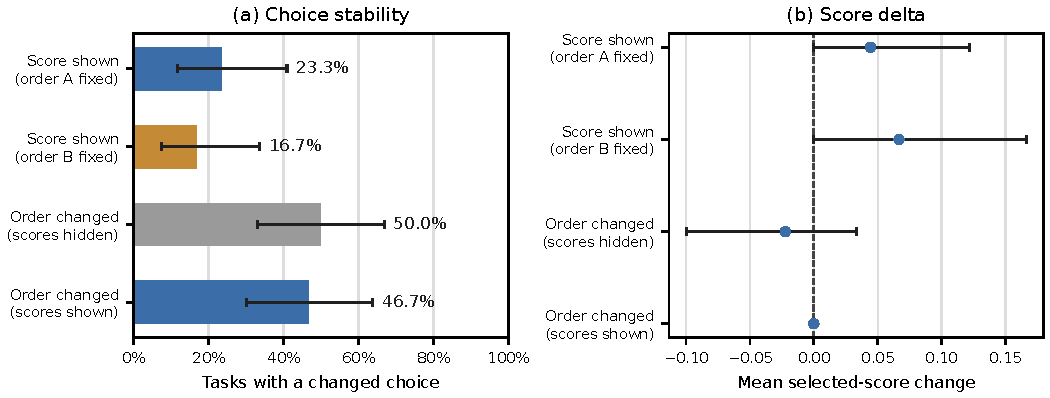
\includegraphics[width=\textwidth]{factorial-audit.pdf}
\caption{Matched interface contrasts. Panel (a) gives the fraction of tasks with a changed selected
slot and Wilson 95\% intervals. Panel (b) gives the mean selected-rubric-score change with paired-task
bootstrap intervals. The four contrasts come from one order pair.}
\label{fig:results}
\end{figure}

\subsection{Score exposure changes choices under both orders}

With order A fixed, score exposure changed the selected candidate on
\ScoreAChoiceChanged{} of \ScoreAChoicePairs{} tasks and changed selected answer content on the same
number of tasks. Under order B, both counts were \ScoreBChoiceChanged{} of
\ScoreBChoicePairs. All changed score-exposure choices therefore represented different answer text.
The observed proportions, \ScoreAChoiceRate{} and \ScoreBChoiceRate, differ descriptively across the
two orders, but the overlapping intervals and single order pair do not support a tested interaction.

The rubric-score changes were sparse: order A had \ScoreAScoreIncreased{} increases,
\ScoreAScoreUnchanged{} ties, and \ScoreAScoreDecreased{} decreases; order B had
\ScoreBScoreIncreased{} increases, \ScoreBScoreUnchanged{} ties, and \ScoreBScoreDecreased{}
decreases. The mean changes were \ScoreAScoreDelta{} (CI \ScoreAScoreDeltaCI) and
\ScoreBScoreDelta{} (CI \ScoreBScoreDeltaCI). These are changes in the selected candidate's rubric
score, not evidence that the selected answer is better in an independent sense.

\subsection{Order changes choices even without scores}

When both arms withheld scores, changing order changed the selected slot on
\OrderNoScoreChoiceChanged{} of \OrderNoScoreChoicePairs{} tasks and selected answer content on
\OrderNoScoreContentChanged. The mean rubric-score change was \OrderNoScoreScoreDelta{} (CI
\OrderNoScoreScoreDeltaCI), with \OrderNoScoreScoreIncreased{} increase,
\OrderNoScoreScoreUnchanged{} ties, and \OrderNoScoreScoreDecreased{} decrease. One slot change selected
byte-identical content.

When both arms showed scores, order changed the selected slot on \OrderScoreChoiceChanged{} of
\OrderScoreChoicePairs{} tasks and answer content on \OrderScoreContentChanged.
None of the \OrderScoreChoiceChanged{} visible-score order changes selected byte-identical content. The selected rubric score
was unchanged in every paired task
(\OrderScoreScoreUnchanged/\OrderScoreScorePairs), so score-visible reordering moved among equally
scored choices in this sample.

\subsection{Ties explain why a rubric delta can miss a choice change}

The coarse outcome was already visible in the candidate pool:
\AllTiedInstrumentTasks{} of \DesignTasks{} tasks had the same deterministic rubric score for all
three candidates. Table~\ref{tab:ties} stratifies the score-exposure contrasts. Score exposure changed
the selected slot in \OrderAAllTiedChoiceChanged{} of \OrderAAllTiedTasks{} all-tied tasks under order
A, and in \OrderBAllTiedChoiceChanged{} of \OrderBAllTiedTasks{} under order B.

\begin{table}[H]
\centering
\small
\begin{tabular}{@{}lccc@{}}
\toprule
Score-exposure contrast & All candidates tied & Nontrivial score variation & Total \\
\midrule
Order A fixed & \OrderAAllTiedChoiceChanged/\OrderAAllTiedTasks & \OrderAVariedChoiceChanged/\OrderAVariedTasks & \ScoreAChoiceChanged/\ScoreAChoicePairs \\
Order B fixed & \OrderBAllTiedChoiceChanged/\OrderBAllTiedTasks & \OrderBVariedChoiceChanged/\OrderBVariedTasks & \ScoreBChoiceChanged/\ScoreBChoicePairs \\
\bottomrule
\end{tabular}
\caption{Slot changes after exposing scores, stratified by whether the three frozen rubric scores
were all equal. The all-tied stratum has no numerical reason to prefer one candidate under the
published score, yet the selector sometimes moved between candidates.}
\label{tab:ties}
\end{table}

The score-visible instrument check was active: both score-visible arms chose a top-scored candidate
in \ExposedTop/\ExposedSlots{} arm-task slots, including \ExposedNontiedTop/\ExposedNontiedSlots{}
slots with nontrivial score variation. The all-tied selections account for many of the remaining
slots because every candidate is top-scored by definition. This check establishes that the displayed
scores reached the selector; it does not identify a cognitive mechanism for the all-tied changes.

\section{Discussion}

\paragraph{Selection is part of the reported evaluation.}
The candidate answers were fixed, but the selected candidate index changed after score visibility or
order changed. A pipeline that reports only the chosen candidate's score can therefore hide an
interface dependence that remains visible when the full choice record is retained. The appropriate
unit of analysis includes the candidate pool, the selector, and the presentation interface.

\paragraph{Choice changes and score changes are different outcomes.}
Score exposure changed choices under both orders, but the deterministic rubric changed on few tasks.
That pattern follows from the large all-tied stratum: moving from one candidate to another need not
change the rubric. Reporting only a mean score would miss most of the observed interface sensitivity,
while reporting only choice instability would overstate what is known about answer quality.

\paragraph{Order requires an explicit control.}
The order-only contrast changed slots and answer content while scores remained hidden. This is
consistent with the broader position-bias literature \citep{shi2024judgingjudges}; the present result
adds a matched record for this selector and task sample. It also shows why score exposure must be
evaluated at a fixed order. Comparing one hidden-order arm with a score-visible arm in a different
order would combine both factors.

\paragraph{The rubric is an outcome, not a referee.}
This benchmark's deterministic evaluator records whether required content appears in a response.
It can make many candidates tie and cannot establish whether a response's reasoning is sound. The
paper therefore does not convert a rubric delta into a quality claim, and a zero mean delta does not
show that the interface manipulation was harmless.

\section{Limitations}

\begin{enumerate}
\item \textbf{One model pair and one order pair.} The generator and selector aliases are fixed, and
only two candidate permutations are observed. The study does not estimate an average over models or
all permutations.
\item \textbf{One deterministic selection per cell.} The design measures sensitivity to the prompt
interface in this configuration; it does not estimate run-to-run variance of a stochastic selector.
\item \textbf{A coarse local benchmark.} Most tasks have an all-tied candidate pool, and the rubric is
not independent ground truth. The sample is a development subset, not a fresh or hidden evaluation.
\item \textbf{No population inference.} Wilson and bootstrap intervals describe uncertainty over this
frozen task sample. They do not repair the single-model, single-order design.
\item \textbf{Model aliases were not logged per response.} Post-run local records identify the
installed model digests, but the runner did not persist a digest with every call.
\item \textbf{No claim about upstream harness benefit.} The experiment evaluates how a selector
responds to interface factors. It does not establish that any harness variant improves task
performance.
\end{enumerate}

\section{Conclusion}

On a frozen \DesignTasks-task candidate pool, both score visibility and candidate order changed the
selector's chosen candidate. Score exposure changed selected answer content on
\ScoreAContentChanged{} tasks under order A and \ScoreBContentChanged{} under order B. Order changed
the selected slot on \OrderNoScoreChoiceChanged{} tasks without scores and
\OrderScoreChoiceChanged{} with scores. Slot changes selecting byte-identical content numbered
\OrderNoScoreSameContentSlot{} without scores and \OrderScoreSameContentSlot{} with scores.

The rubric often could not distinguish the candidates: \AllTiedInstrumentTasks{} of
\DesignTasks{} tasks had an all-tied pool. This makes choice-level auditing necessary even when a
score-level comparison looks stable. The result is local and descriptive; its practical value is the
separated, hash-checked record and the demonstration that score exposure and order should be reported
as distinct interface factors.

\section*{Data and Code Availability}

This draft is accompanied by a local reproducibility directory containing the frozen source record,
raw candidate manifest, independent score recomputation, order-contract check, deterministic
analysis, generated figure, and verification scripts. Appendix~\ref{app:repro} records the
reproduction checks. No public repository or DOI is claimed in this draft. The source run is
identified by SHA-256:
\begin{flushleft}\ttfamily\small\SourceDigest\end{flushleft}
The recomputed analysis is identified by:
\begin{flushleft}\ttfamily\small\AnalysisDigest\end{flushleft}
Appendix~\ref{app:excluded} records the legacy claims excluded from this revision.

\appendix

\section{Reproduction Record}\label{app:repro}

The experiment command, model aliases, source record, and environment observations were captured
alongside the manuscript. The analysis can be regenerated from the source JSON without calling a
model. The following checks are separate evidence files:

\begin{itemize}
\item raw candidate manifest: 90 expected files, 90 captured, zero missing;
\item order repair: \OriginalHardOrderMismatchTasks/\DesignTasks{} original order-B mismatches
  identified, only the affected arm replayed, and \HardRepairPickChangedTasks{} picks changed;
\item score recomputation: 90 stored scores reproduced exactly, zero mismatches;
\item order contract: the factorial mapping is present and the two orders differ on
  \OrderContractDiffer/\DesignTasks{} tasks;
\item content comparison: selected raw answers were hashed before the slot-change counts were
  interpreted;
\item manuscript values: generated from the analysis JSON and the captured run configuration.
\end{itemize}

The deterministic analysis was run twice and produced byte-identical JSON. The original manuscript
and all earlier revision directories were preserved.

\section{Claims Excluded from This Revision}\label{app:excluded}

Earlier drafts contained a judge-inflation comparison, Cohen's \(\kappa\) as an effect measure, and a
simulation that treated selection benefit as bias. Those analyses are excluded here. The
judge-inflation records did not consistently bind judged answers to their declared source files; the
kappa comparison did not have an effect-test null hypothesis; and the simulation's estimand mixed
selected-object quality with cross-task strategy value. None of those legacy values is used in the
abstract, results, figures, or conclusion of this manuscript.

This revision also omits the earlier benchmark-defect extrapolation and any claim that anonymity
removes presentation effects. The present result is narrower: for one fixed candidate pool, two
selection-interface factors changed choices, while the deterministic rubric often did not register a
score change.

\bibliographystyle{plainnat}
\bibliography{references}

\end{document}
